%
% $RCSfile: observer.tex,v $
%
% Copyright (C) 2002-2008. Christian Heller.
%
% Permission is granted to copy, distribute and/or modify this document
% under the terms of the GNU Free Documentation License, Version 1.1 or
% any later version published by the Free Software Foundation; with no
% Invariant Sections, with no Front-Cover Texts and with no Back-Cover
% Texts. A copy of the license is included in the section entitled
% "GNU Free Documentation License".
%
% http://www.cybop.net
% - Cybernetics Oriented Programming -
%
% http://www.resmedicinae.org
% - Information in Medicine -
%
% Version: $Revision: 1.1 $ $Date: 2008-08-19 20:41:07 $ $Author: christian $
% Authors: Christian Heller <christian.heller@tuxtax.de>
%

\subsubsection{Observer}
\label{observer_heading}
\index{Observer Pattern}
\index{Publisher-Subscriber Pattern}
\index{Callback Event Handling}
\index{Model View Controller Pattern}
\index{MVC}
\index{Bidirectional Dependency}
\index{Circular Reference}

Another pattern that found wide application is the \emph{Observer} \cite{gamma1995},
an often-used synonym for which is \emph{Publisher-Subscriber}. It provides a
notification mechanism for all objects that registered as \emph{Observer} at a
\emph{Subject} in whose state changes they are interested, leading to an automatic
update of all dependent objects (figure \ref{observer_figure}).

\begin{figure}[ht]
    \begin{center}
        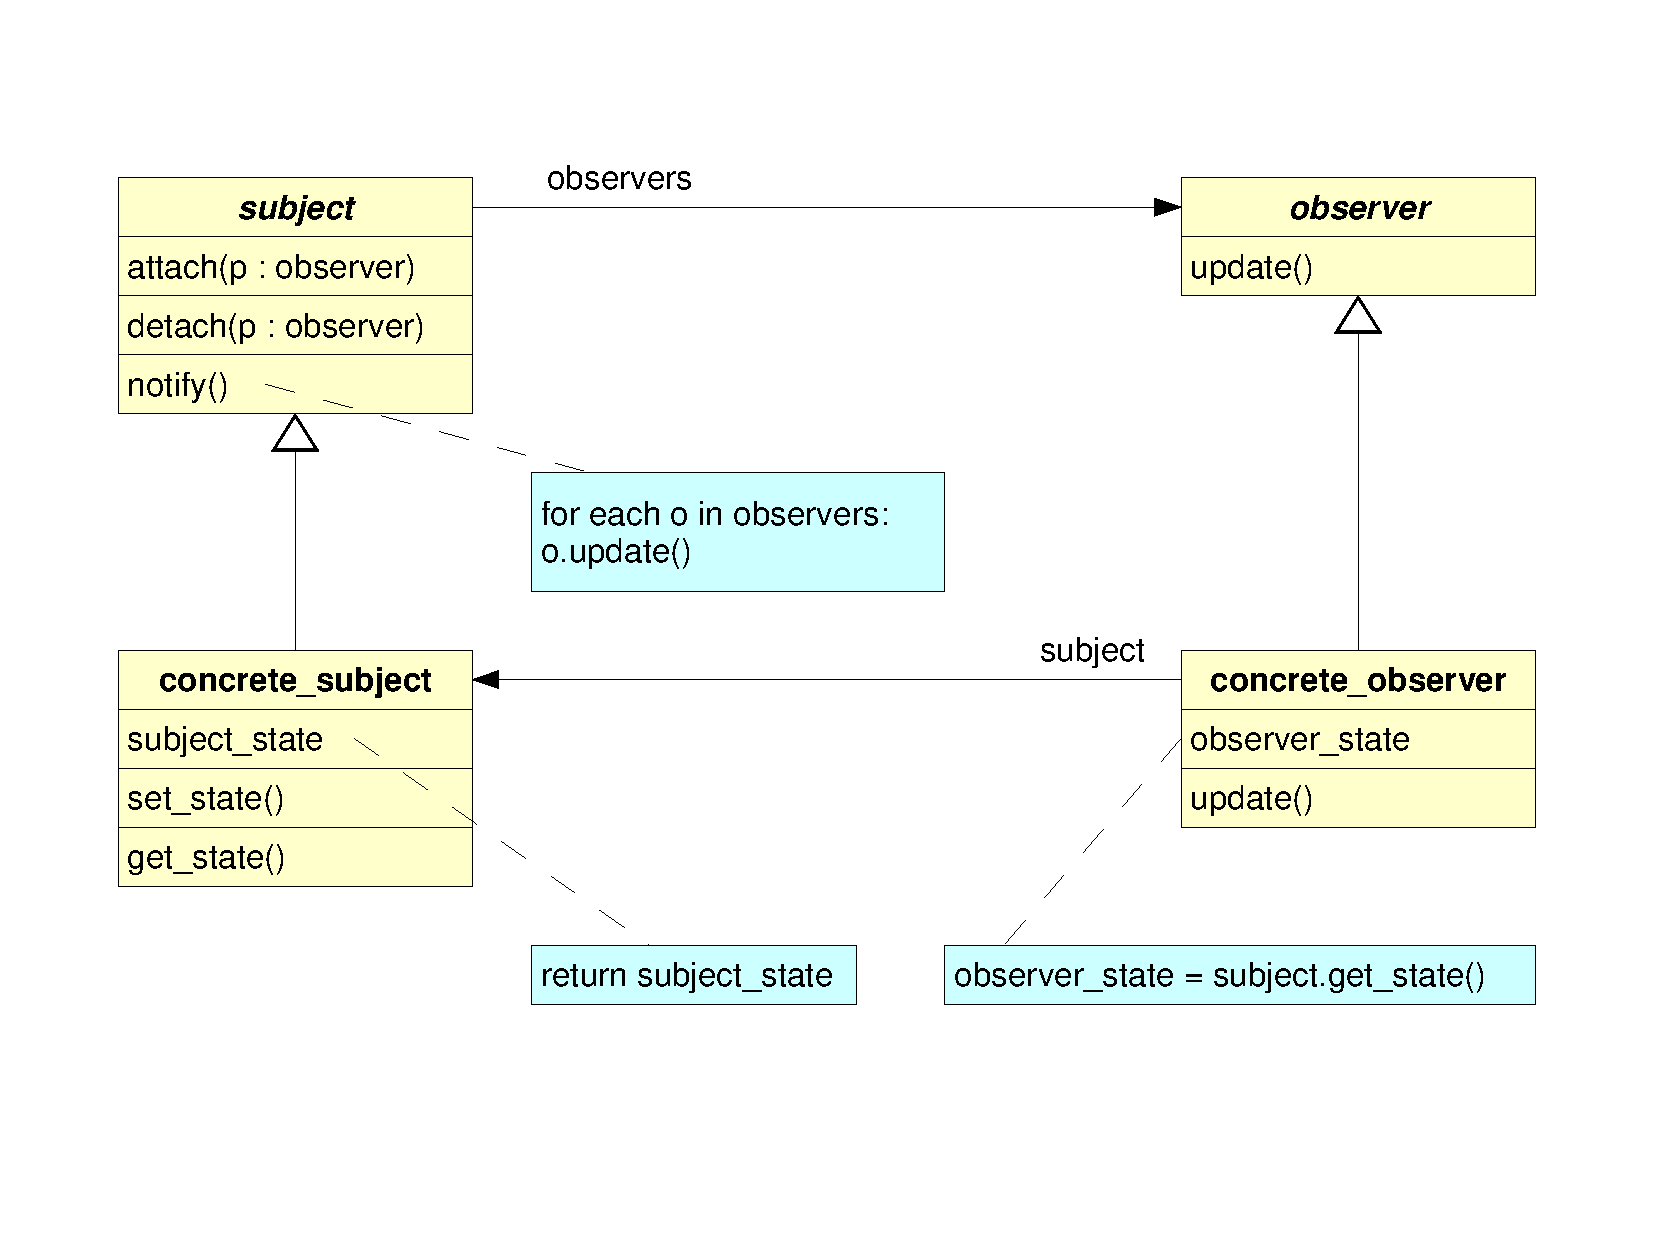
\includegraphics[scale=0.3,angle=-90]{graphic/observer.pdf}
        \caption{Observer Pattern}
        \label{observer_figure}
    \end{center}
\end{figure}

Similar notification mechanisms are used for \emph{Callback} event handling in
frameworks (section \ref{framework_heading}), where the framework core calls
functionality of its extensions. The \emph{Model View Controller-} (MVC)
(section \ref{model_view_controller_heading}) uses the \emph{Observer} pattern
to let the model notify its observing views about necessary updates (figure
\ref{mvcobserver_figure}). The disadvantage of the \emph{Observer} pattern is
that it relies on bidirectional dependencies, so that circular references can
occur, when a system is not programmed very carefully.

\begin{figure}[ht]
    \begin{center}
        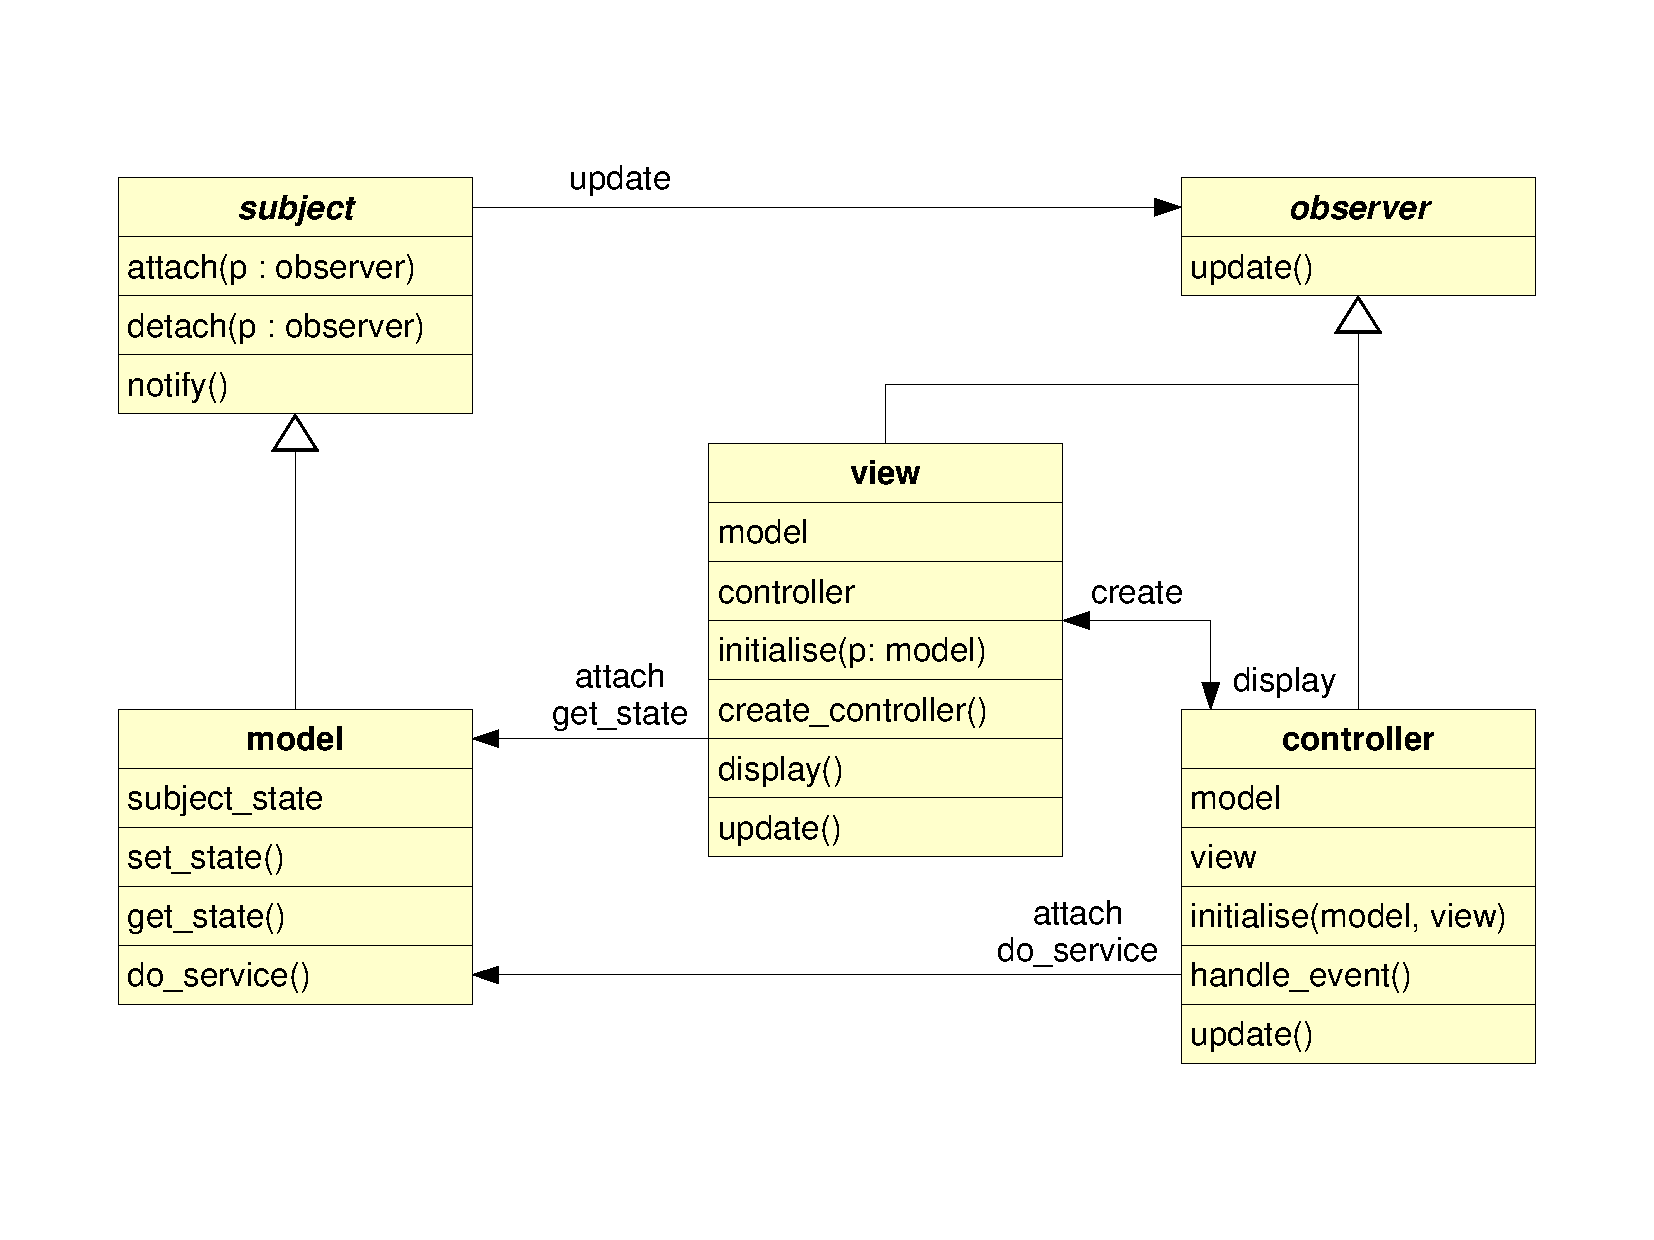
\includegraphics[scale=0.3,angle=-90]{graphic/mvcobserver.pdf}
        \caption{MVC- using Observer Pattern}
        \label{mvcobserver_figure}
    \end{center}
\end{figure}

The new pattern systematics presented in chapter \ref{knowledge_schema_heading}
classifies the \emph{Observer} as not recommendable pattern. The language and
interpreter described in chapters \ref{cybernetics_oriented_language_heading}
and \ref{cybernetics_oriented_interpreter_heading} do avoid its usage.
